\documentclass[12pt, a4paper]{article}
\usepackage{../notesheets}
\usepackage{epsdice}

\newcommand{\Var}{\operatorname{Var}}
%%%%%%%%%%%%%%%%%%%%%%%%%%%%%%%%%%%%%%%%%%%%%%%%%%
\author{Math 1220}
\title{Notesheet. Section 10.3: Normal Distributions} 
\date{}

\begin{document}
\maketitle
\nameline
%%%%%%%%%%%%%%%%%%%%%%%%%%%%%%%%%%%%%%%%%%%%%%%%%%
\begin{defi}
  The general \de{normal probability density function} with mean
  \(\mu\) and standard deviation \(\sigma\) is defined to be \[
    f(x) = \hspace{1in}
  \]
  A \de{normal variable} is a RV \(X\) with PDF given by a normal
  probability density function. \\
  Note, the \de{standard normal distribution} is the normal
  probability density function with \(\mu = 0\)
  and \(\sigma=1\), thus giving simpler equation \[
    f(x) = \hspace{1in}
  \]
  The \de{standard normal variable} is the RV \(Z\) with PDF given by
  the standard normal distribution.
\end{defi}
\vspace{-0.3in}
\begin{thrm}
  The graph of a normal distribution is called a \de{normal curve},
  which looks like the following graph: \\
  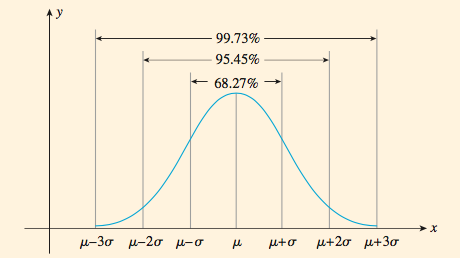
\includegraphics[scale=0.7]{images/normal-curve}
\end{thrm}
\vspace{-1in}
\begin{rmk}
  Since the integrals associated to the normal distribution are
  difficult to compute by hand, traditionally one would consult a
  table, often called a \de{Z table}. A small part of the Z table is
  here: \\
  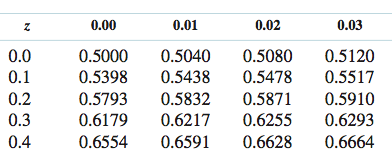
\includegraphics[scale=0.6]{images/z-table}\\
  You can find a copy of the Z table on the internet or Appendix C of
  the textbook.
\end{rmk}
\begin{ex}
  Using the Z table above, find \(P(Z \leq 0.23), P(0 < Z < 0.23)\),
  and \(P(Z > 0.23)\). Also, using the Z table above, find a number
  \(m\) such that \(P(Z \leq m)  = 0.5517\). 
\end{ex}
\begin{thrm}
  Given a normal variable \(X\) with mean \(\mu\) and standard
  deviation \(\sigma\), then \[
    \frac{X-\mu}{\sigma} = \hspace{3in}
  \]
  and so \[
    P(X < b) = \hspace{3in}
  \]
\end{thrm}
\begin{ex}
  If \(X\) is a normal variable with mean \(10\) and standard
  deviation \(3\), find the value of \(m\) such that \(P(X<m) = 0.591\). 
\end{ex}
\vspace{-0.5in}
\begin{ex}
  Assume that
  \begin{itemize}
  \item The weights of M\&M's are normally distributed with mean
    \(9\) grams and standard deviation \(1\) gram.
  \item The weights of Skittles are normally distributed with mean
    \(10\) gram and standard deviation \(2\) grams.
  \end{itemize}
  What is more likely?
  \begin{enumerate}
  \item A randomly chosen M\&M weights \(>10\) grams.
  \item A randomly chosen Skittle weights \(>10\) grams.
  \end{enumerate}

\end{ex}
%%%%%%%%%%%%%%%%%%%%%%%%%%%%%%%%%%%%%%%%%%%%%%%%%% 
\end{document}
